\section{Kalman Filter simulation}

Consider a simple linear system with known analytical solution: a projectile launched with an initial velocity, falling under the influence of a constant gravity, with no air resistance.
The gravitational acceleration is treated as a deterministic input.
The $y$ axis is taken as normal to the ground, leading to the following true dynamics for the position states $x,y$ and velocities $v_x,v_y$:
\begin{align}
\dot{x} = v_x \\
\dot{v_x} = 0 \\
\dot{y} = v_y \\
\dot{v_y} = -g \\
\xk \equiv \begin{bmatrix} x\k & v_x\k & y\k & v_y\k \end{bmatrix}^T
\end{align}

The initial states are chosen such that $v_x = v_y \approx 70.7$ m/s, and the gravitational acceleration is taken as a constant $9.81$ m/s$^2$.
The system is discretized with a simple Euler integration model at $\Delta T = 0.01$ seconds, leading to the following discrete-time process model:

\begin{equation}
\xkone = \begin{bmatrix}
1 & \Delta T & 0 & 0\\
0 & 1 & 0 & 0\\
0 & 0 & 1 & \Delta T\\
0 & 0 & 0 & 1
\end{bmatrix}\xk + 
\begin{bmatrix}
0 \\ 0 \\ 0 \\ -\Delta T
\end{bmatrix} g
\end{equation}

Note that no explicit process noise is included in the dynamics.
However, the simulated states are evaluated using the analytical solution, which leads to a discretization error due to the use of Euler integration.
This discretization error is modeled as a zero-mean process with the following covariance:

\begin{equation}
\Qk = \mathrm{diag}\begin{bmatrix} \Delta T^{0.25} & \Delta T & \Delta T & \Delta T \end{bmatrix}
\end{equation}

This covariance was tuned experimentally to produce more consistent filter outputs.
The measurement matrix is taken simply to be identity, with linear measurements of the full state.
The measurement covariance matrix is diagonal with each measurement having variance 10.
Python simulation results are now presented.

\begin{figure}[tb!]
\centering
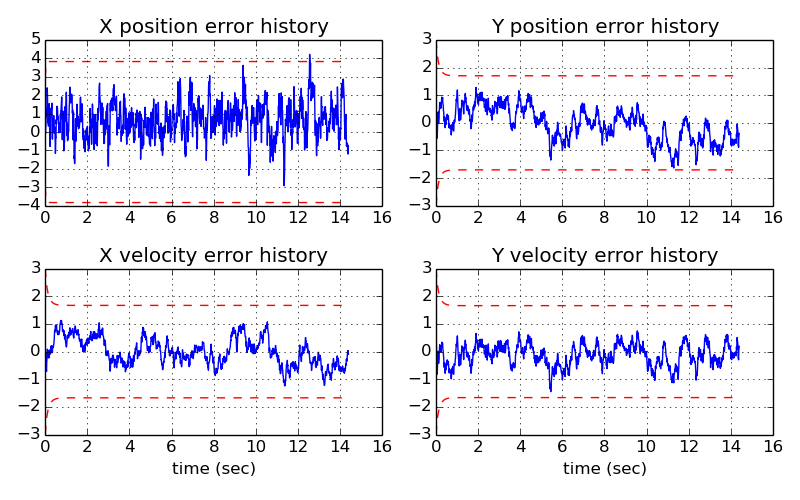
\includegraphics[width=\textwidth]{kf_errors}
\caption{Kalman filter errors relative to truth. $3\times$ the square root of covariance diagonals plotted in red for reference.}
\label{fig:kf_errors}
\end{figure}

\begin{figure}[tb!]
\centering
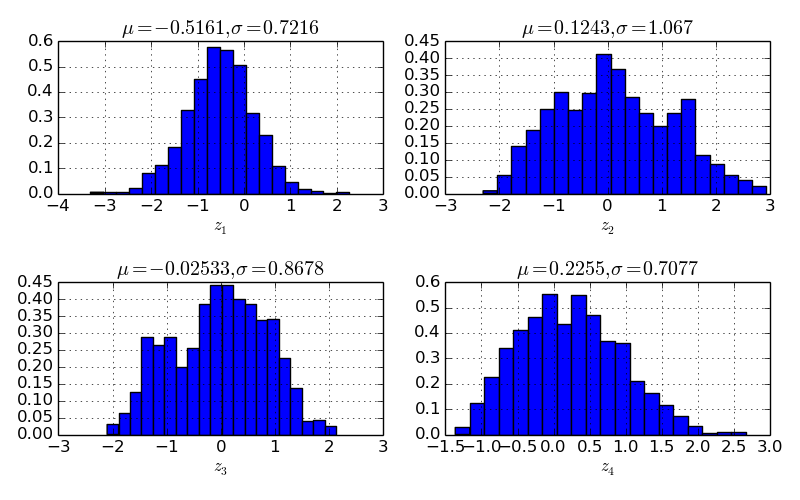
\includegraphics[width=\textwidth]{kf_consistency}
\caption{Histograms of normalized filter states.}
\label{fig:kf_consistency}
\end{figure}

For brevity, we show only the filter tracking errors (Fig. \ref{fig:kf_errors}) and consistency histograms (Fig. \ref{fig:kf_consistency}).
Fig. \ref{fig:kf_errors} shows the difference between the filter states and true states at each moment in time.
Three times the square root of the covariance diagonal elements is plotted as a metric of filter accuracy and consistency.
(For a independent random variables, these would be $3\sigma$ bounds; in this case, we consider these bounds as approximations, which retain physical significance.)
The filter appears to be somewhat conservative, since the errors are typically less than the $3\sigma$ approximations.
However, the $x$ position history shows a bias.
This bias likely is largely attributable to the use of first-order discretized integration.

For Fig. \ref{fig:kf_consistency}, the filter errors are regularized to states $\vec{z}$ having expected mean and covariance $0,1$, according to the following transform: $\vec{z}(k) \equiv \ten{P(k)}^{1/2}(\vec{x}(k)-\vec{\hat{x}}(k))$.
If the filter is consistent, the regularized states $\vec{z}$ should be zero-mean and have unit variance.
In Fig. \ref{fig:kf_consistency}, histograms of the regularized states are plotted.
Note that states $z_1,z_2,z_3,z_4$ correspond approximately to x position, x velocity, y position, and y velocity.
It is clear that the states are approximately Gaussian but with some error.
In particular, the $z_1$ and $z_4$ states exhibit a noticeable bias and the filter is conservative, because the actual variance is less than 1.
The $z_2$ and $z_4$ states are more consistent.

Overall, the filter implementation is imperfect, but adequate for the purposes of demonstrating the basics of the Kalman Filter.
The following section explores advanced topics in nonlinear sequential estimation.